% !TEX TS-program = xelatex
% !TeX program = xelatex
% !TEX encoding = UTF-8
% !TEX spellcheck = fr

%=====================================================================
\ifx\wholebook\relax\else
	\documentclass{KodeBook}
	% !TEX TS-program = xelatex
% !TeX program = xelatex
% !TEX encoding = UTF-8
% !TEX spellcheck = fr

%\usepackage[T1]{fontenc}

%\usepackage[pdftex]{graphicx}

%\usepackage{listingsutf8}
%\usepackage{xcolor}
%\usepackage{times}
\usepackage{array}
\usepackage{natbib}
\usepackage{lscape}%to flip tables in a page
\usepackage{pdflscape}
\usepackage{longtable}
\usepackage{tabu}
\usepackage{wrapfig}
\usepackage{colortbl}
\usepackage{alltt}
\usepackage[french,lined]{algorithm2e}

\renewcommand{\cite}[1]{\citep{#1}}

%\usepackage[english]{babel}

\bibliographystyle{engdnat}%unsrtnat, plainnat

%\usepackage{pgf-umlcd}





\hypersetup{
	pdfkeywords={TALN; TAL; langue},
	pdfsubject={intelligence artificielle; traitement automatique de langages naturels}
}

\renewcommand{\UrlFont}{\ttfamily\footnotesize}

\DeclareAcronym{taln}{
	short = TALN ,
	long  = traitement automatique de langages naturels,
	class = abbrev
}

\DeclareAcronym{tal}{
	short = TAL ,
	long  = traitement automatique des langues,
	class = abbrev
}

\DeclareAcronym{ia}{
	short = IA ,
	long  = intelligence artificielle,
	class = abbrev
}

\DeclareAcronym{ibm}{
	short = IA ,
	long  = international business machines,
	class = abbrev
}

\DeclareAcronym{darpa}{
	short = DARPA ,
	long  = Defense Advanced Research Projects Agency,
	class = abbrev
}

\DeclareAcronym{ipa}{
	short = IPA ,
	long  = intelligent personal assistant,
	class = abbrev
}

\DeclareAcronym{iva}{
	short = IVA ,
	long  = intelligent virtual assistant,
	class = abbrev
}

\DeclareAcronym{ipa2}{
	short = IPA ,
	long  =  International Phonetic Alphabet,
	class = abbrev
}

%\makeglossaries

%\newacronym{oop}{OOP}{Object-oriented programming} 

	\begin{document}
		\mainmatter
	
\fi
%=====================================================================
\changegraphpath{../img/syntaxe/}
\chapter{Analyse syntaxique}

\begin{introduction}
	\lettrine{L}{e} 
\end{introduction} 

\begin{exampleblock}{Exemple d'une phrase en français}
	\begin{center}
		\Large\bfseries
		L'élève a écrit une solution avec un stylo. 
		
		L'élève a écrit une solution avec une explication.
	\end{center}
\end{exampleblock}

\begin{itemize}
	\item Qui a écrit la solution ?
	\item Quel instrument a-t-on utilisé pour l'écriture ?
	\begin{itemize}
		\item Un stylo ? Une explication ?
	\end{itemize}
	\item Est-ce qu'on a écrit d'autres choses en plus de la solution ?
	\begin{itemize}
		\item Un stylo ? Une explication ?
	\end{itemize}
	\item Comment avez-vous déduit ça ?
\end{itemize}

%===================================================================================
\section{Structures syntaxiques}
%===================================================================================

\begin{itemize}
	\item Une phrase peut être bien formée syntaxiquement mais pas sémantiquement 
	\begin{itemize}
		\item Ex. \expword{Les idées vertes et non colorées dorment furieusement.}
	\end{itemize}
	\item Plusieurs théories 
	\begin{itemize}
		\item La grammaire générative et transformationnelle : Ex. \expword{Grammaire générative et transformationnelle (TTG)}
		\item La grammaire de dépendance 
		\item La grammaire catégorique
		\item Les grammaires stochastiques
		\item Les approches fonctionnelles de la grammaire
	\end{itemize}
	
\end{itemize}

\subsection{Annotation constituante}

\begin{itemize}
	\item Les mots d'une phrase ont chacun \keyword{une catégorie grammaticale}
	\begin{itemize}
		\item Ex. \expword{Le/DET cours/NOM est/VP intéressant/ADJ}
	\end{itemize}
	\item Un ou plusieurs mots de certaines catégories forment \keyword{un syntagme}
	\begin{itemize}
		\item Ex. \expword{[Le/DET cours/NOM ]\textsubscript{NP} [est/VP intéressant/ADJ VP]\textsubscript{VP}}
	\end{itemize}
\end{itemize}

\begin{center}
	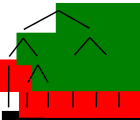
\includegraphics[width=0.4\textwidth]{../img/intro/gram_const.pdf}
\end{center}

Grammaires à contexte libre (CFG)
\begin{minipage}{.68\textwidth}
	\begin{itemize}
		\item $G <\Sigma, N, P, S>$ est une grammaire.
		\item $\Sigma$ est le vocabulaire : ensemble des symboles terminaux
		\begin{itemize}
			\item \expword{$\Sigma$ = \{le, petit, chat, mange, un, poisson, ...\}}
		\end{itemize}
		\item $V$ est l'ensemble des  variables : symboles non terminaux 
		\begin{itemize}
			\item \expword{$N$ = \{S, NP, VP, DET, N, ADJ, ...\}}
		\end{itemize}
	\end{itemize}
\end{minipage}
\begin{minipage}{.3\textwidth}
	\hgraphpage{humour-chomsky.jpg}
\end{minipage}

\begin{itemize}
	\item $S \in N$ est l'axiome.
	\item $P$ est l'ensemble des règles de production.
	\item Les règles sont de la forme $A \rightarrow \beta \text{ avec } A \in N,\, \beta \in (\Sigma \cup N)^*$
	\begin{itemize}
		\item \expword{S \textrightarrow NP VP}
		\item \expword{NP \textrightarrow DET ADJ N \textbar\ DET N}
		\item \expword{VP \textrightarrow V NP}
	\end{itemize}
\end{itemize}

CFG probabiliste (PCFG)

\begin{itemize}
	\item $G <\Sigma, N, P, S>$ est une grammaire.
	\item Les règles sont de la forme $A \rightarrow \beta\, [p] \text{ avec } A \in N,\, \beta \in (\Sigma \cup N)^*$
	\item $p$ est la probabilité d'occurrence de la règle
	\item Cette probabilité est estimée à partir d'un corpus annoté (\keyword{TreeBank})
\end{itemize}

\begin{block}{Estimation des probabilité des règles}
	\[
	P(A \rightarrow \beta | A) = \frac{C(A \rightarrow \beta)}{C(A)}
	\]
\end{block}

\subsection{Annotation fonctionnelle}

\begin{itemize}
	\item Un mot ou plus remplissent \keyword{une fonction syntaxique}
	\begin{itemize}
		\item Ex. \expword{sujet, objet, etc.}
	\end{itemize}
	\item Les liens syntaxiques entre les mots d'une phrase sont appelés : \keyword{dépendances}
	\begin{itemize}
		\item Ex. \expword{Le chat mange un poisson} : ici ``chat" est \expword{le sujet} du verbe ``mange"
	\end{itemize}
	\item Une relation de dépendance relie un mot appelé \keyword{tête syntaxique} avec un autre appelé \keyword{dépendant}
\end{itemize}

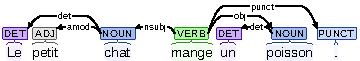
\includegraphics[width=\textwidth]{../img/intro/gram-dep_.pdf}

Relations de dépendance
\begin{table}
	\rowcolors{2}{lightblue}{lightyellow}
	\begin{tabular}{p{.2\textwidth}p{.35\textwidth}p{.35\textwidth}}
		\rowcolor{darkblue}
		\textcolor{white}{Dép. de base} & \textcolor{white}{Description} & \textcolor{white}{Exemple}\\
		nsubj & sujet nominal & Le \underline{people} \textbf{gagne}\\
		obj & objet direct & On \textbf{présente} le \underline{cours}\\
		iobj & objet indirect & Il \underline{m'}\textbf{envoie}\\
		csubj & sujet propositionnel & \underline{Suivre} le cours \textbf{permet} ...\\
		
		\rowcolor{darkblue}
		\textcolor{white}{Dép. des noms} & \textcolor{white}{Description} & \textcolor{white}{Exemple}\\
		amod & modificateur adjectival & La \textbf{fille} \underline{modeste}\\
		det & déterminant & \underline{La} \textbf{fille}\\
		nmod & modificateur nominal & Le \underline{résultat} de la \textbf{course}\\
		nummod & modificateur numérique & J'ai mangé \underline{3} \textbf{bonbons}\\
		
	\end{tabular}
	\caption{Quelques relations de dépendances universelles de Stanford \cite{2014-de-marneffe-al} (\url{https://universaldependencies.org/u/dep/index.html})}
\end{table}

%===================================================================================
\section{Analyse des constituants}
%===================================================================================

\begin{itemize}
	\item La grammaire à contexte libre : le système formel le plus utilisé pour modéliser la structure constituante
	\item Analyse 
	\begin{itemize}
		\item \optword{ascendante} : à partir des mots de la phrase, on essaye de trouver les catégories grammaticales. Ensuite, les syntagmes qui génèrent une combinaison des catégories et des syntagmes. On fait ça jusqu'à arriver à \keyword{S}
		\item \optword{descendante} : à partir de \keyword{S}, on cherche les règles qui génèrent la phrase. Ceci en se basant sur des mots pour guider la génération.
	\end{itemize}
\end{itemize}

\begin{center}
	\begin{tabular}{|p{.25\textwidth}|p{.3\textwidth}|p{.3\textwidth}|}
		\hline
		& Classique & Statistique \\
		\hline
		Ascendante & \optword{CKY}, LR & \optword{CKY probabiliste}\\
		\hline
		Descendante & Early, LL, Descente récursive  & \\
		\hline
	\end{tabular}
\end{center}

\subsection{Algorithme CKY}

\begin{itemize}
	\item Algorithme de \keyword{Cocke-Kasami-Younger}
	\item Analyse ascendante
	\item Prérequis : Forme normale de Chomsky
\end{itemize}

\begin{definition}[FNC : Forme normale de Chomsky]
	\[
	A \rightarrow  B C \text{ où } A, B, C \in N
	\]
	
	\[
	A \rightarrow w \text{ où } w \in \Sigma
	\]
\end{definition}

Reconnaissance d'une phrase
\begin{block}{CKY : Reconnaissance d'une phrase}
	\scriptsize\vspace{-3pt}
	\begin{algorithm}[H]
		\Donnees{une grammaire $G <\Sigma, N, P, S>$ en FNC; une phrase $w = w_1 \ldots w_n$}
		\Res{$T[n, n], B[n, n, |N|]$}
		
		\Pour{$ i = 1 \ldots n$}{ 
			$T[i-1, j] \leftarrow \{  A / (A \rightarrow w_j) \in P \} $\;
		}
		
		\Pour{$ j = 2 \ldots n$ }{%\tcc*{Iitialiser le diagonal}
			\Pour{$ i = 0 \ldots (n - j) $}{
				\Pour{$ k = (i+1) \ldots (i + j -1 ) $}{
					\PourTous{$A$ tel que $(A \rightarrow B C) \in P $ et $B \in T[i, k]$ et $C \in T[k, i+j]$}{ 
						$T[i, i+j] \leftarrow T[i, i+j] \cup \{A\}$ ;
						$B[i, i+j, A] \leftarrow B[i, i+j, A] \cup \{(B, C, k)\}$ \;
					}
				}
			}
		}
		
		\Si{$``S" \notin T[0, n] $} {
			Erreur ``La phrase n'a pas été reconnue"\;
		}
		
		\Retour $T, B$ \;
		\vspace{-3pt}
	\end{algorithm}
\end{block}

Construction de l'arbre
\begin{block}{CKY : Construction de l'arbre}
	\scriptsize\vspace{-3pt}
	\begin{algorithm}[H]
		\SetKwFunction{FConst}{Construire}
		\SetKwProg{Fn}{Fonction}{\\Début}{Fin}
		
		\Donnees{$T[n, n], B[n, n, |N|]$}
		\Res{Arbre syntaxique}
		
		\eSi{$``S" \notin T[0, n] $} {
			\Retour $\varnothing$ \;
		}{
			\Retour \FConst{$S, 0, n$}\;
		}
		
		\Fn{\FConst{$A, i, j$}}{
			
			\eSi{j = i + 1}{
				\Retour $A$\;
			}{
				$ (B, C, k) \leftarrow Choisir(B[i, j, A]) $\;
				\Retour (\FConst{$B, i, k$}, \FConst{$C, k, j$})\;
			}
		}
		
		
		%		\vspace{-3pt}
	\end{algorithm}
\end{block}

Exercice
\begin{exampleblock}{Exemple d'une grammaire}
	\begin{itemize}
		\item S \textrightarrow\ NP VP 
		\item S \textrightarrow\ VP 
		\item VP \textrightarrow V NP
		\item NP \textrightarrow\ DET ADJ N \textbar\ DET N \textbar\ PRON 
		\item PRON \textrightarrow\ je \textbar\ tu \textbar\ il \textbar\ elle
		\item V \textrightarrow\ forme \textbar\ veut \textbar\ mange 
		\item DET \textrightarrow\ un \textbar\ une \textbar\ la \textbar\ le
		\item ADJ \textrightarrow\ petite \textbar\ grand \textbar\ bleu 
		\item N \textrightarrow\ petite \textbar\ forme \textbar\ phrase \textbar\ chat \textbar\ poisson
	\end{itemize}
\end{exampleblock}\vspace{-6pt}

\begin{itemize}
	\item Analyser la phrase suivante en utilisant CKY 
	\item \expword{la petite forme une petite phrase}
\end{itemize}

Remarques
\begin{minipage}{.53\textwidth}
	\begin{itemize}
		\item L'arbre syntaxique résultante est binaire. Mais, dans la réalité elle doit suivre la grammaire conçue par les syntacticiens
		\begin{itemize}
			\item Ajouter une étape de post-traitement pour récupérer l'arbre originale
			\item Laisser les productions unitaires et modifier l'algorithme CKY afin de les accepter
		\end{itemize}
		\item Problème d'ambigüité syntaxique 
		\begin{itemize}
			\item Ex. \expword{Je mange du riz avec une fourchette.} et \expword{Je mange du riz avec de la viande.}
			%		\item 
		\end{itemize}
	\end{itemize}
\end{minipage}

\subsection{Algorithme CKY probabiliste}
\begin{itemize}
	\item $G<\Sigma, N, P, S>$ est une grammaire probabiliste
	\item Les nouvelles règles créées par transformation en FNC ont une probabilité égale à $1$
	\item $w = w_1 \ldots w_n$ est un mot à analyser 
	\item $T$ est un arbre syntaxique 
	\item $P(T, w) = \prod\limits_{(A_i \rightarrow \beta_i) \in T} P(A_i \rightarrow \beta_i)$ est la probabilité d'un arbre syntaxique étant donné le mot analysé $w$
	\item $\hat{T}(w) = \arg\max\limits_{T(w)} P(T, w) $ est l'arbre syntaxique le plus adéquat pour analyser le mot $w$
\end{itemize}

Reconnaissance d'une phrase
\begin{block}{CKY probabiliste : Reconnaissance d'une phrase}
	\scriptsize\vspace{-3pt}
	\begin{algorithm}[H]
		\Donnees{une grammaire probabiliste $G <\Sigma, N, P, S>$ en FNC; une phrase $w = w_1 \ldots w_n$}
		\Res{$T[n, n, |N|], B[n, n, |N|]$}
		
		\Pour{$ i = 1 \ldots n$}{ 
			\PourTous{$A / (A \rightarrow w_j) \in P$}{
				$T[i-1, j, A] \leftarrow P(A \rightarrow w_j)$\;
			}
		}
		
		\Pour{$ j = 2 \ldots n$ }{%\tcc*{Iitialiser le diagonal}
			\Pour{$ i = 0 \ldots (n - j) $}{
				\Pour{$ k = (i+1) \ldots (i + j -1 ) $}{
					%					\PourTous{$A$ tel que $(A \rightarrow B C) \in P $ et $B \in T[i, k]$ et $C \in T[k, i+j]$}{ 
					$T[i, i+j, A] \leftarrow \max\limits_{A \rightarrow B C \in P} P(A \rightarrow B C) * T[i, k, B] * T[k, i+j, C]$ \;
					$B[i, i+j, A] \leftarrow (B, C, k)$\;
					%					}
				}
			}
		}
		
		\texttt{// Si $``S" \notin T[0, n] $ : Erreur}
		%		\Si{} {
		%			Erreur ``La phrase n'a pas été reconnue"\;
		%		}
		
		\Retour $T, B$ \;
		\vspace{-3pt}
	\end{algorithm}
\end{block}

%===================================================================================
\section{Analyse des dépendances}
%===================================================================================

\begin{minipage}{.6\textwidth}
	\begin{itemize}
		\item \optword{Analyse basée sur les transitions} 
		\begin{itemize}
			\item \textbf{Configuration} :  $C = (\sigma, \beta, A)$ où $\sigma$ est une pile, $\beta$ est le tampon (buffer) d'entrée et $A$ est la liste des arcs créés
			\item $C_{initiale} = ([ROOT], w, \emptyset)$
			\item $C_{finale} = ([ROOT], \varnothing, A)$
			%		\item Un ensemble d'actions possibles
		\end{itemize}
	\end{itemize}
\end{minipage}
\begin{minipage}{.38\textwidth}
	\hgraphpage{transitions.pdf}
\end{minipage}

\begin{minipage}{.6\textwidth}
	\begin{itemize}
		\item \optword{Analyse basée sur les graphes}
		\begin{itemize}
			\item \textbf{Graphe} : $G = (V, E)$ où $V$ est l'ensemble de nœuds (mots) et $E$ l'ensemble d'arcs (relations de dépendance)
			\item \textbf{Résultat} : $T = (V, F)$ un sous-graphe de $G$ représentant les relations de dépendance
		\end{itemize}
	\end{itemize}
\end{minipage}
\begin{minipage}{.38\textwidth}
	\hgraphpage{graphe.pdf}
\end{minipage}

\subsection{Par transition}

\begin{minipage}{.6\textwidth}
	\begin{itemize}
		\item \textbf{Configuration} :  $C = (\sigma, \beta, A)$
		\begin{itemize}
			\item $\sigma$ est une pile
			\item $\beta$ est le tampon (buffer) d'entrée
			\item $A$ est la liste des arcs créés (dépendances)
			\item $C_{initiale} = ([ROOT], w, \emptyset)$
			\item $C_{finale} = ([ROOT], \varnothing, A)$
		\end{itemize}
	\end{itemize}
\end{minipage}
\begin{minipage}{.38\textwidth}
	\hgraphpage{transitions.pdf}
\end{minipage}

\begin{itemize}
	\item \textbf{Transition} : passer d'un état vers un autre en utilisant des actions sur
	\begin{itemize}
		\item $\sigma$ : empiler ou dépiler un mot
		\item $\beta$ : retirer un mot ou ajouter un au début
		\item $A$ : ajouter une dépendance entre 2 mots
	\end{itemize}
	\item \textbf{Oracle} : un système qui décide la transition suivante
\end{itemize}

Algorithme d'analyse
\begin{itemize}
	\item Le système ``$Oracle$" choisit une transition ``$t$"
	\item La fonction ``$Appliquer$" exécute ``$t$" sur la configuration
\end{itemize}

\begin{block}{Analyse des dépendances par transitions}
	\begin{algorithm}[H]
		\Donnees{Le mot à analyser $w= w_1 w_2 \ldots w_n$}
		\Res{Liste des dépendances $A$}
		
		$C \leftarrow (\sigma=[ROOT], \beta = w, A = \emptyset)$\;
		
		
		\Tq{$\sigma \ne [ROOT]$ OU $\beta \ne \varnothing$}{
			$t \leftarrow Oracle(C)$\;
			$C \leftarrow Appliquer(C, t)$\;
		}
		
		\Retour $A$ \;
	\end{algorithm}
\end{block}

Système Oracle (entraînement)
\begin{itemize}
	\item Le système Oracle apprend à inférer la transition $\hat{t}$ étant donné
	\begin{itemize}
		\item la configuration actuelle $ C = (\sigma, \beta, A) $
		\item l'ensemble $T$ des transactions possibles
		\item une fonction $\Psi$ qui calcule un score en utilisant sur des caractéristiques basées sur la configuration 
		\item un texte annoté (TreeBank)
	\end{itemize}
	\[ \hat{t} = \arg\max\limits_{t \in T} \Psi (t, C, w; \theta) \]
	
	\item Le texte annoté doit être transformé à une séquence de transactions
	\item Pour entraîner l'Oracle, on utilise l'algorithme d'analyse 
	\item La fonction $\Psi$ peut être MaxEnt (le plus utilisé), SVM ou les réseaux de neurones
\end{itemize}

\begin{itemize}
	\item \textbf{La pile $\sigma$}
	\begin{itemize}
		\item Le mot dans le sommet de la pile
		\item La catégorie grammaticale de ce mot
	\end{itemize}
	
	\item \textbf{Le tampon d'entrée $\beta$}
	\begin{itemize}
		\item Les trois premiers mots
		\item Leurs catégories grammaticales
	\end{itemize}
	
	\item \textbf{La liste des dépendances $A$}
	\begin{itemize}
		\item Les dépendances qui ont été estimées
	\end{itemize}
	
	\item \textbf{La phrase analysée $w$}
	\begin{itemize}
		\item La distance entre le mot du sommet de la pile et le premier mot dans le tampon (nombre des mots entre eux dans la phrase $w$)
	\end{itemize}
	
\end{itemize}

Arc-standard (transitions possibles)
\begin{itemize}
	\item \optword{SHIFT} : Déplacer le premier élément dans le tampon vers la pile 
	\[ (\sigma, w_i|\beta, A) \Rightarrow  (\sigma|w_i, \beta, A) \]
	
	\item \optword{ARC-LEFT} : Établir un arc du premier élément dans le tampon vers le sommet de la pile
	\[ (\sigma|w_i, w_j|\beta, A) \Rightarrow  (\sigma, w_j|\beta, A \cup \{w_j \rightarrow w_i \}) \] 
	
	\item \optword{ARC-RIGHT} : Établir un arc du sommet de la pile vers le premier élément dans le tampon
	\[ (\sigma|w_i, w_j|\beta, A) \Rightarrow  (\sigma, w_i|\beta, A \cup \{w_i \rightarrow w_j \}) \] 
\end{itemize}

\begin{figure}
	\hgraphpage{exp-arc-std_.pdf}
	\caption{Exemple de dérivations non étiquetées de la phrase ``\expword{they like bagels with lox}" en utilisant Arc-standard \cite{2018-eisenstein}}
\end{figure}

Arc-Eager (transitions possibles)

\begin{itemize}
	\item \optword{SHIFT} est le même que ``Arc-standard"
	
	\item \optword{ARC-LEFT} : Établir un arc du premier élément dans le tampon vers le sommet de la pile
	\[ (\sigma|w_i, w_j|\beta, A) \xRightarrow{\forall w_k (w_k \rightarrow w_i) \notin A}  (\sigma, w_j|\beta, A \cup \{w_j \rightarrow w_i \}) \] 
	
	\item \optword{ARC-RIGHT} : Établir un arc du sommet de la pile vers le premier élément dans le tampon
	\[ (\sigma|w_i, w_j|\beta, A) \Rightarrow  (\sigma|w_i w_j, \beta, A \cup \{w_i \rightarrow w_j \}) \] 
	
	\item \optword{REDUCE} : Dépiler un mot s'il a déjà un parent
	\[ (\sigma|w_i, \beta, A) \xRightarrow{\exists w_k (w_k \rightarrow w_i) \in A} (\sigma, \beta, A) \] 
	%	\[ (\sigma|w_i, \beta, \mathcal{A}) \overset{\exists w_k (w_k \rightarrow w_i) \in \mathcal{A}}{\Longrightarrow} (\sigma, \beta, \mathcal{A}) \] 
\end{itemize}

\begin{figure}
	\hgraphpage{exp-arc-eager_.pdf}
	\caption{Exemple de dérivations non étiquetées de la phrase ``\expword{they like bagels with lox}" en utilisant Arc-eager \cite{2018-eisenstein}}
\end{figure}

\subsection{Par graphe}

\begin{minipage}{.6\textwidth}
	\begin{itemize}
		\item Analyse basée sur les graphes
		\begin{itemize}
			\item Graphe : $G = (V, E)$ où $V$ est l'ensemble de nœuds (mots) et $E$ l'ensemble d'arcs (relations de dépendance)
			\item Résultat : $T = (V, F)$ un sous-graphe de $G$ représentant les relations de dépendance
		\end{itemize}
	\end{itemize}
\end{minipage}
\begin{minipage}{.38\textwidth}
	\hgraphpage{graphe.pdf}
\end{minipage}

\begin{itemize}
	\item $\Psi$ est une fonction de score, $ \mathcal{T}(G) $ est l'espace des arbres de dépendance possibles sur $G$
	\[ \hat{T} = \arg\max\limits_{T \in \mathcal{T}(G)} \Psi(T, w; \theta) \]
	\item Ce score est calculé en se basant sur le score de chaque arc $\psi$
	\[ \Psi(T, w; \theta) = \sum_{e \in F / T = (V, F)} \psi(e, w; \theta) \]
\end{itemize}

Score et entraînement
\begin{itemize}
	\item Le score d'un arc dépend de certaines caractéristiques (d'ordre $K$)
	\[ \psi(e, w; \theta) = \sum_{k = 1}^{K} \theta_k f_k(e, w)  \]
	
	\item Quelques caractéristiques 
	\begin{itemize}
		\item Le mot de l'entête, sa catégorie grammaticale, son lemme, ses préfixes et suffixes
		\item La direction de l'arc
		\item La distance entre l'entête et le dépendant
		\item \ldots
	\end{itemize}
	
\end{itemize}

Analyse de Chu-Liu/Edmonds
\begin{itemize}
	\item On ajoute un nœud (ROOT) avec des arcs vers tous le reste des nœuds 
	\item Les arcs sont pondérés où le poids d'un arc $e$ est $G.p(e)$
	\item On construit un \keyword{Arbre couvrant} de poids maximal
	\item \keyword{Arbre couvrant} : Un sous-graphe acyclique maximal où tous les nœuds sont connectés et il n'y a pas plus qu'un arc entrant vers un nœud
	\item \optword{Contracter} : une fonction qui fusionne deux nœuds $u$ et $v$ composant un cycle $C$
	\begin{itemize}
		\item $\forall e = (u', v) \in E : G.p(e) \leftarrow G.p(e) - G.p((u, v)) $
		\item $\forall e = (v', u) \in E : G.p(e) \leftarrow G.p(e) - G.p((v, u)) $
	\end{itemize}
	\item \optword{Etendre} : une fonction qui désassemble les deux nœuds $u$ et $v$ d'un cycle $C$. L'arc qui enfreint la condition ``\textit{pas de deux arcs entrants}" est supprimé
\end{itemize}

\begin{block}{Analyse de Chu-Liu-Edmonds : Arbre couvrant de poids maximal}
	\scriptsize\vspace{-6pt}
	\begin{algorithm}[H]
		\Donnees{un graphe pondéré $G = (V, E)$, $ ROOT $}
		\Res{un arbre couvrant $T = (V, F)$}
		
		\SetKwFunction{ACM}{ArbreCouvrantMax}
		\SetKwProg{Fn}{Fonction}{}{Fin Fonction} 
		
		\Fn{\ACM{$G, ROOT$}}{
			
			$F \leftarrow \emptyset$\;
			
			\PourTous{$ v \in V$}{ 
				$meilleurInArc \leftarrow \arg\max_{e = (u, v) \in E} G.p(e) $;
				$F \leftarrow F \cup meilleurInArc$\;
				\PourTous{$e = (u, v) \in E$}{ 
					$ G.p(e) \leftarrow G.p(e) - G.p(meilleurInArc) $\;
				}
				\eSi{$T = (V, F)$ est un arbre couvrant}{
					\Retour $T$ \;
				}{
					$C \leftarrow$ un cycle de $F$;
					$G' \leftarrow Contracter(G, C)$\;
					$T' \leftarrow ArbreCouvrantMax(G', ROOT)$;
					$T \leftarrow Etendre(T', C)$\;
					\Retour $T$ \;
				}
			}
			
		}
		\vspace{-3pt}
	\end{algorithm}\vspace{-3pt}
\end{block}

\begin{figure}
	\centering
	\hgraphpage[.8\textwidth]{exp-graphe_.pdf}
	\caption{Exemple d'un graphe de la phrase ``Book a flight" \cite{2019-jurafsky-martin}}
\end{figure}


\begin{discussion}



\end{discussion}

%=====================================================================
\ifx\wholebook\relax\else
% \cleardoublepage
% \bibliographystyle{../use/ESIbib}
% \bibliography{../bib/RATstat}
	\end{document}
\fi
%=====================================================================
